%%%%%%
%
% $Autor: Sandesh Nonavinakere Sunil, Mahadas Gangadhar Anand $
% $Datum: today $
% $Directory: ML24-05-Keyword-Spotting-with-an-Arduino-Nano-33-BLE-Sense\report\Contents\en\Application.tex $
% $Version: 2 $
% $Autor: Sandesh Nonavinakere Sunil, Mahadas Gangadhar Anand $
% $Review date: today $
%
%%%%%%

\chapter{Keyword Spotting}

\section{Keyword Spotting}

Keyword spotting is a branch of speech recognition that deals with the identification of special speech commands or ``keywords'' in utterances. With a small footprint size, keyword spotting has a wide scope of applications, such as robotics, virtual assistants, and vehicle mounted electronics. In the field of retail, using ‘keywords’ can enable a customer to get updates on orders or be directed to the customer help centers with simple keyword responses such as ‘yes’ and ‘no’. Virtual assistants use a variety of small special speech commands such as ‘Hey Siri’ or ‘Alexa’ to switch from sleep mode to wake up mode and respond to requests by the user. In the field of robotics, service robots can be directed to move in specific directions such as ‘left’, ‘right’, ‘backward’, ‘forward’ or execute actions using other keywords. For keyword spotting to be efficient, it is important that we achieve a good accuracy of speech recognition, low-latency and be able to run in computationally constrained environments (such as mobile devices). \cite{rai:2023,Abbas:2023}

\section{Problem Statement}

The scope of this project is to build a keyword spotting application using the Arduino Nano 33 BLE Sense. The selected keywords for recognition are "Yes" and "No, We have decided to implement a Convolutional Neural Network (CNN) architecture for this task due to its proven ability to extract relevant features from audio data effectively.
Our task involves building the application from scratch, which includes gathering audio data directly from the device's onboard microphone and augmenting it with samples from the Google Speech Command dataset. This collected data will be preprocessed and used to train the machine learning algorithm. Finally, the trained model will be deployed and tested on the Arduino Nano 33 BLE Sense to ensure accurate keyword recognition under real-world conditions.

\section{Data Acquisition}

The critical component of any Machine Learning Workflow is the dataset. Once we have decided on specific keywords, in our case "Yes" and "No, we can take advantage of the Google speech dataset which has keywords (with +1,000 samples each), such as yes, no, stop, and go etc.

Although we have a lot of data from google dataset, collecting some words spoken by us is advised. Creating a dataset with data captured by the same type of sensor is essential. In the case of sound, this is optional because what we will classify is, in reality, audio data. \cite{Harvard:2024}     

\begin{center}

	
\includegraphics[width=0.7\textwidth]{KeywordSpotting/AudioCapture.jpg}
	\captionof{figure}{New Audio data capture \cite{Harvard:2024} }
	\label{fig:New Audio data capture}
\end{center}

\section{Data Quantity}

The volume of data available for training significantly influences a model's performance. Larger datasets can enhance a model's ability to generalize and improve accuracy. However, merely increasing data volume without considering quality may not yield better results. A study on data governance in materials science emphasizes the need for a synergistic approach that combines domain knowledge with data quantity to accelerate machine learning applications.\cite{Liu:2023}

\section{Data Quality}

High-quality data is essential for training reliable machine learning models. Poor-quality data can introduce biases, reduce model performance, and lead to overfitting. A survey on data quality dimensions and tools for machine learning highlights that improving data quality can be more efficient than merely increasing data quantity.\cite{Zhou:2024}

\section{Data Relevance}

The relevance of data pertains to how well the training data represents the problem domain. Irrelevant or redundant data can confuse the learning process, leading to suboptimal models. Ensuring that the data aligns closely with the specific application enhances model effectiveness. A survey of data quality requirements in machine learning systems underscores the importance of relevant data in building effective models.\cite{Priestley:2023}

\section{Outliers}

Outliers are those data points that are slightly different from the
rest of the dataset. They are often abnormal observations that skew
the data distribution, and arise due to inconsistent data entry, or
erroneous observations.\cite{C:2022}

This could lead to less effective and less useful models.
But dealing with outliers often requires domain expertise, and none of
the outlier detection techniques should be applied without
understanding the data distribution and the use case.

\begin{center}
	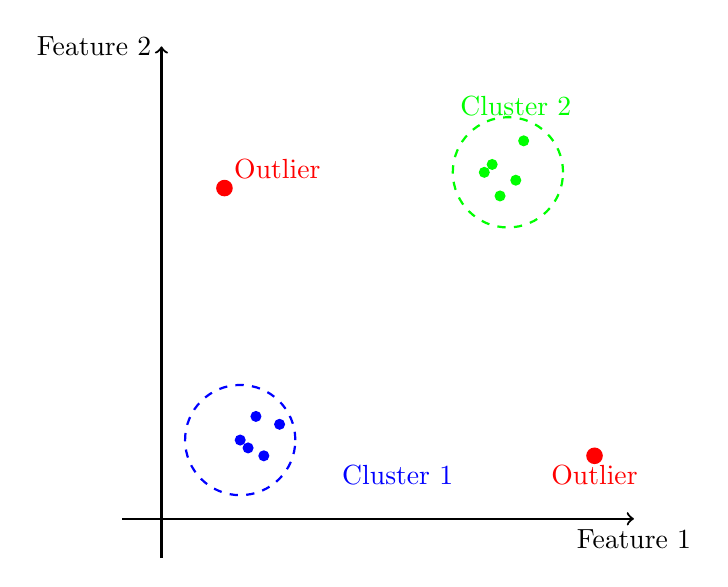
\begin{tikzpicture}
		% Draw axes
		\draw[->, thick] (-0.5, 0) -- (6, 0) node[below] {Feature 1};
		\draw[->, thick] (0, -0.5) -- (0, 6) node[left] {Feature 2};
		
		% Normal points cluster 1
		\foreach \x/\y in {1/1, 1.2/1.3, 1.5/1.2, 1.3/0.8, 1.1/0.9} {
			\fill[blue] (\x,\y) circle (2pt);
		}
		\node[below, blue] at (3,0.8) {Cluster 1};
		
		% Normal points cluster 2
		\foreach \x/\y in {4.2/4.5, 4.5/4.3, 4.6/4.8, 4.3/4.1, 4.1/4.4} {
			\fill[green] (\x,\y) circle (2pt);
		}
		\node[above, green] at (4.5,5) {Cluster 2};
		
		% Highlight outliers
		\fill[red] (0.8,4.2) circle (3pt);
		\node[above right, red] at (0.8,4.2) {Outlier};
		
		\fill[red] (5.5,0.8) circle (3pt);
		\node[below, red] at (5.5,0.8) {Outlier};
		
		% Add annotations
		\draw[thick, dashed, blue] (1,1) circle (0.7cm); % Cluster 1 boundary
		\draw[thick, dashed, green] (4.4,4.4) circle (0.7cm); % Cluster 2 boundary
	\end{tikzpicture}
	\captionof{figure}{Outlier Detection}
	\label{fig:Outlier Detection}
\end{center}

The goal of outlier detection is to remove the points—which are truly
outliers—so you can build a model that performs well on unseen test
data.\cite{C:2022}

\section{Anomalies}


Keyword spotting (KWS) systems are designed to detect specific words or phrases within continuous speech. However, they often encounter anomalies that can compromise their performance. Understanding these anomalies is crucial for developing robust KWS applications.

\newpage
\begin{enumerate}
	\item \textbf{Acoustic Variability and Noise Interference}
	
	KWS systems are susceptible to variations in acoustic environments, such as background noise, reverberation, and differing speaker characteristics. These factors can lead to false detections or missed keywords. Research has focused on enhancing noise robustness through novel loss functions and training strategies. \cite{Lopez:2021}
	
	\item \textbf{Catastrophic Forgetting in Continual Learning}
	
	When KWS models are updated with new data, they may experience catastrophic forgetting, where previously learned keywords are forgotten. Progressive continual learning approaches have been proposed to address this challenge, enabling models to retain prior knowledge while integrating new information. \cite{Huang:2022}
	
	\item \textbf{Resource Constraints on Edge Devices}
	
	Deploying KWS systems on edge devices with limited computational resources presents challenges in maintaining accuracy and efficiency. Explorations into neural network architectures tailored for edge devices aim to balance performance with resource limitations. \cite{Bushur:2023}
	
	\item \textbf{False Alarms and Detection Latency}
	
	Achieving high wake-up accuracy with low false alarm rates in real-time systems is challenging, especially under computational constraints. Techniques such as successive refinement have been developed to reduce false alarms while maintaining prompt keyword detection. \cite{Saidutta:2023}
	
	\item \textbf{Multi-Talker and Overlapping Speech Scenarios}
	
	In environments with multiple speakers, distinguishing the target keyword becomes complex. Text-aware speech separation methods have been introduced to enhance KWS performance in multi-talker situations by separating overlapping speech based on textual clues.\cite{Li:2024}
	
	\item \textbf{Anomalies in Textual Data}
	
	Beyond audio, anomalies can also occur in textual data associated with KWS systems. Detecting such anomalies is essential for maintaining system integrity. A systematic review of machine learning techniques for text anomaly detection provides insights into addressing these challenges.\cite{Boutalbi:2023}
\end{enumerate}

Addressing these anomalies is vital for the development of reliable and efficient keyword spotting applications across diverse environments and platforms. 



\section{Constraints}

Outliers in data for a Keyword Spotting (KWS) application arise when input audio deviates significantly from the patterns used during model training. Here’s a detailed explanation of the listed constraints:

\begin{enumerate}
	\item \textbf{Distance of the User from the Microphone:} 
	\begin{itemize}
		\item The further a user is from the microphone, the lower the signal strength, resulting in reduced clarity of the spoken keyword. 
		\item Background noise and environmental sounds might overpower the user's voice when distant, leading to detection errors.
		\item Variations in distance affect the audio amplitude, which may be outside the range the model has been trained to recognize.
	\end{itemize}
	
	\item \textbf{Voice Strength:}
	\begin{itemize}
		\item Soft-spoken users may produce audio signals with low amplitude, causing the keyword to be masked by noise or not detected at all.
		\item On the other hand, users with very loud voices might cause distortion in the audio, especially if the microphone has a limited dynamic range.
		\item Such variability makes it challenging for the model to generalize effectively.
	\end{itemize}
	
	\item \textbf{Speaking Accent:}
	\begin{itemize}
		\item Differences in accents can lead to varied pronunciations of the same keyword, altering the phonetic structure.
		\item Models trained on a limited dataset might not include sufficient samples of diverse accents, causing misclassification or failure to detect keywords spoken with certain accents.
	\end{itemize}
	
	\item \textbf{Speech Clarity:}
	\begin{itemize}
		\item Users with unclear or slurred speech, possibly due to health conditions, fatigue, or hurried speech, might not produce a well-defined representation of the keyword.
		\item Background noises, reverberation, or microphone quality can exacerbate the lack of clarity, making it harder for the system to isolate and detect the keyword.
	\end{itemize}
	
	\item \textbf{Pronunciation Techniques:}
	\begin{itemize}
		\item Different users may emphasize syllables differently or have unique ways of enunciating sounds, leading to variability in how the keyword is pronounced.
		\item For instance, regional variations may involve omitting or adding phonemes, which the model might not recognize as corresponding to the intended keyword.
	\end{itemize}
\end{enumerate}
Addressing these constraints requires a robust dataset with diverse examples for training, along with data augmentation techniques to simulate variations. Additionally, integrating noise suppression, distance normalization, and accent adaptation mechanisms can help mitigate the impact of these outliers in a KWS application.

\section{Code with simple example}

Below is a simple example to read microphone data:


\begin{lstlisting}[caption={Code with simple example}, label={lst:simple_example}]
	/**
	* @file microphone_example.ino
	* @brief Example code to read data from a PDM microphone.
	* 
	* This code initializes a PDM microphone and reads audio data in real-time,
	* printing the data to the serial monitor.
	*/
	
	#include <Arduino.h>
	#include <PDM.h>
	
	/**
	* @brief Setup function to initialize the PDM microphone and Serial communication.
	* 
	* The function sets up the Serial port for debugging and initializes the PDM
	* microphone with one channel and a sampling rate of 16 kHz.
	*/
	void setup() {
		// Initialize Serial communication at 115200 baud rate.
		Serial.begin(115200);
		
		// Initialize the PDM library with 1 channel and a 16 kHz sample rate.
		if (!PDM.begin(1, 16000)) {
			Serial.println("Failed to initialize PDM!");
			while (1); // Infinite loop to halt execution on initialization failure.
		}
		
		Serial.println("PDM Microphone initialized.");
	}
	
	/**
	* @brief Main loop to process and print PDM microphone data.
	* 
	* The loop checks if there is available audio data in the PDM buffer. If data
	* is available, it reads the data into a buffer, processes it, and prints it
	* to the Serial monitor.
	*/
	void loop() {
		// Check the number of bytes available in the PDM buffer.
		int bytesAvailable = PDM.available();
		
		if (bytesAvailable) {
			// Allocate a buffer to store the audio data (16-bit samples).
			int16_t buffer[bytesAvailable / 2];
			
			// Read the data from the PDM microphone into the buffer.
			PDM.read(buffer, bytesAvailable);
			
			// Process and print each audio sample to the Serial monitor.
			for (int i = 0; i < bytesAvailable / 2; i++) {
				Serial.println(buffer[i]);
			}
		}
	}
\end{lstlisting}


